% Options for packages loaded elsewhere
\PassOptionsToPackage{unicode}{hyperref}
\PassOptionsToPackage{hyphens}{url}
%
\documentclass[
  man,floatsintext]{apa7}
\usepackage{amsmath,amssymb}
\usepackage{iftex}
\ifPDFTeX
  \usepackage[T1]{fontenc}
  \usepackage[utf8]{inputenc}
  \usepackage{textcomp} % provide euro and other symbols
\else % if luatex or xetex
  \usepackage{unicode-math} % this also loads fontspec
  \defaultfontfeatures{Scale=MatchLowercase}
  \defaultfontfeatures[\rmfamily]{Ligatures=TeX,Scale=1}
\fi
\usepackage{lmodern}
\ifPDFTeX\else
  % xetex/luatex font selection
\fi
% Use upquote if available, for straight quotes in verbatim environments
\IfFileExists{upquote.sty}{\usepackage{upquote}}{}
\IfFileExists{microtype.sty}{% use microtype if available
  \usepackage[]{microtype}
  \UseMicrotypeSet[protrusion]{basicmath} % disable protrusion for tt fonts
}{}
\makeatletter
\@ifundefined{KOMAClassName}{% if non-KOMA class
  \IfFileExists{parskip.sty}{%
    \usepackage{parskip}
  }{% else
    \setlength{\parindent}{0pt}
    \setlength{\parskip}{6pt plus 2pt minus 1pt}}
}{% if KOMA class
  \KOMAoptions{parskip=half}}
\makeatother
\usepackage{xcolor}
\usepackage{graphicx}
\makeatletter
\def\maxwidth{\ifdim\Gin@nat@width>\linewidth\linewidth\else\Gin@nat@width\fi}
\def\maxheight{\ifdim\Gin@nat@height>\textheight\textheight\else\Gin@nat@height\fi}
\makeatother
% Scale images if necessary, so that they will not overflow the page
% margins by default, and it is still possible to overwrite the defaults
% using explicit options in \includegraphics[width, height, ...]{}
\setkeys{Gin}{width=\maxwidth,height=\maxheight,keepaspectratio}
% Set default figure placement to htbp
\makeatletter
\def\fps@figure{htbp}
\makeatother
\setlength{\emergencystretch}{3em} % prevent overfull lines
\providecommand{\tightlist}{%
  \setlength{\itemsep}{0pt}\setlength{\parskip}{0pt}}
\setcounter{secnumdepth}{-\maxdimen} % remove section numbering
% Make \paragraph and \subparagraph free-standing
\ifx\paragraph\undefined\else
  \let\oldparagraph\paragraph
  \renewcommand{\paragraph}[1]{\oldparagraph{#1}\mbox{}}
\fi
\ifx\subparagraph\undefined\else
  \let\oldsubparagraph\subparagraph
  \renewcommand{\subparagraph}[1]{\oldsubparagraph{#1}\mbox{}}
\fi
\ifLuaTeX
\usepackage[bidi=basic]{babel}
\else
\usepackage[bidi=default]{babel}
\fi
\babelprovide[main,import]{english}
% get rid of language-specific shorthands (see #6817):
\let\LanguageShortHands\languageshorthands
\def\languageshorthands#1{}
% Manuscript styling
\usepackage{upgreek}
\captionsetup{font=singlespacing,justification=justified}

% Table formatting
\usepackage{longtable}
\usepackage{lscape}
% \usepackage[counterclockwise]{rotating}   % Landscape page setup for large tables
\usepackage{multirow}		% Table styling
\usepackage{tabularx}		% Control Column width
\usepackage[flushleft]{threeparttable}	% Allows for three part tables with a specified notes section
\usepackage{threeparttablex}            % Lets threeparttable work with longtable

% Create new environments so endfloat can handle them
% \newenvironment{ltable}
%   {\begin{landscape}\centering\begin{threeparttable}}
%   {\end{threeparttable}\end{landscape}}
\newenvironment{lltable}{\begin{landscape}\centering\begin{ThreePartTable}}{\end{ThreePartTable}\end{landscape}}

% Enables adjusting longtable caption width to table width
% Solution found at http://golatex.de/longtable-mit-caption-so-breit-wie-die-tabelle-t15767.html
\makeatletter
\newcommand\LastLTentrywidth{1em}
\newlength\longtablewidth
\setlength{\longtablewidth}{1in}
\newcommand{\getlongtablewidth}{\begingroup \ifcsname LT@\roman{LT@tables}\endcsname \global\longtablewidth=0pt \renewcommand{\LT@entry}[2]{\global\advance\longtablewidth by ##2\relax\gdef\LastLTentrywidth{##2}}\@nameuse{LT@\roman{LT@tables}} \fi \endgroup}

% \setlength{\parindent}{0.5in}
% \setlength{\parskip}{0pt plus 0pt minus 0pt}

% Overwrite redefinition of paragraph and subparagraph by the default LaTeX template
% See https://github.com/crsh/papaja/issues/292
\makeatletter
\renewcommand{\paragraph}{\@startsection{paragraph}{4}{\parindent}%
  {0\baselineskip \@plus 0.2ex \@minus 0.2ex}%
  {-1em}%
  {\normalfont\normalsize\bfseries\itshape\typesectitle}}

\renewcommand{\subparagraph}[1]{\@startsection{subparagraph}{5}{1em}%
  {0\baselineskip \@plus 0.2ex \@minus 0.2ex}%
  {-\z@\relax}%
  {\normalfont\normalsize\itshape\hspace{\parindent}{#1}\textit{\addperi}}{\relax}}
\makeatother

% \usepackage{etoolbox}
\makeatletter
\patchcmd{\HyOrg@maketitle}
  {\section{\normalfont\normalsize\abstractname}}
  {\section*{\normalfont\normalsize\abstractname}}
  {}{\typeout{Failed to patch abstract.}}
\patchcmd{\HyOrg@maketitle}
  {\section{\protect\normalfont{\@title}}}
  {\section*{\protect\normalfont{\@title}}}
  {}{\typeout{Failed to patch title.}}
\makeatother

\usepackage{xpatch}
\makeatletter
\xapptocmd\appendix
  {\xapptocmd\section
    {\addcontentsline{toc}{section}{\appendixname\ifoneappendix\else~\theappendix\fi\\: #1}}
    {}{\InnerPatchFailed}%
  }
{}{\PatchFailed}
\usepackage{csquotes}
\usepackage{setspace}
\AtBeginEnvironment{tabular}{\singlespacing}
\AtBeginEnvironment{lltable}{\singlespacing}
\AtBeginEnvironment{tablenotes}{\doublespacing}
\captionsetup[table]{font={stretch=1.5}}
\captionsetup[figure]{font={stretch=1.5}}
\AtBeginDocument{\let\maketitle\relax}
\raggedbottom
\ifLuaTeX
  \usepackage{selnolig}  % disable illegal ligatures
\fi
\IfFileExists{bookmark.sty}{\usepackage{bookmark}}{\usepackage{hyperref}}
\IfFileExists{xurl.sty}{\usepackage{xurl}}{} % add URL line breaks if available
\urlstyle{same}
\hypersetup{
  pdftitle={Socioeconomic status and adolescent brain responses to peer feedback: Testing the impact on negative affect},
  pdfauthor={Brent I. Rappaport1, James E. Glazer1, Lilian Y. Li1, Madeline M. McGregor1, Lili A. Massac2, Katherine Durham2, Randy P. Auerbach2, \& Stewart A. Shankman1},
  pdflang={en-EN},
  hidelinks,
  pdfcreator={LaTeX via pandoc}}

\title{Socioeconomic status and adolescent brain responses to peer feedback: Testing the impact on negative affect}
\author{Brent I. Rappaport\textsuperscript{1}, James E. Glazer\textsuperscript{1}, Lilian Y. Li\textsuperscript{1}, Madeline M. McGregor\textsuperscript{1}, Lili A. Massac\textsuperscript{2}, Katherine Durham\textsuperscript{2}, Randy P. Auerbach\textsuperscript{2}, \& Stewart A. Shankman\textsuperscript{1}}
\date{}


\shorttitle{SES \& brain responses to peer feedback}

\authornote{

The authors made the following contributions. Brent I. Rappaport: Conceptualization, Formal analysis, Writing - Original Draft Preparation, Writing - Review \& Editing; James E. Glazer: Methodology, Writing - Review \& Editing; Lilian Y. Li: Methodology, Writing - Review \& Editing; Madeline M. McGregor: Writing - Review \& Editing; Lili A. Massac: Writing - Review \& Editing; Katherine Durham: Writing - Review \& Editing; Randy P. Auerbach: Conceptualization, Fundind acquisition, Investigation, Methodology, Resources, Supervision, Writing - Review \& Editing; Stewart A. Shankman: Conceptualization, Fundind acquisition, Investigation, Methodology, Resources, Supervision, Writing - Review \& Editing.

Correspondence concerning this article should be addressed to Brent I. Rappaport, 680 N. Lakeshore Drive, Suite 1520, Chicago, IL 60611. E-mail: \href{mailto:brent.rappaport@northwestern.edu}{\nolinkurl{brent.rappaport@northwestern.edu}}

}

\affiliation{\vspace{0.5cm}\textsuperscript{1} Department of Psychiatry, Feinberg School of Medicine, Northwestern University\\\textsuperscript{2} Columbia University}

\begin{document}
\maketitle

\newpage{}

\begin{lltable}

\begin{TableNotes}[para]
\normalsize{\textit{Note.} Note. N=1 excluded for missing group variable. N=3 missing Age. N=1 missing SES. N=2 missing Sex. N=1 missing Hispanic ethnicity. N=1 missing Race. N=3 missing IDAS depression. N=3 missing Lifetime number of stressors. N=3 missing Lifetime stressor severity. * p<.05, ** p<.01, *** p<.001}
\end{TableNotes}

\small{

\begin{longtable}{p{8cm}p{2.5cm}p{2.5cm}p{2cm}p{1.5cm}}\noalign{\getlongtablewidth\global\LTcapwidth=\longtablewidth}
\caption{\label{tab:demoTable}}\\
\toprule
Variable & \multicolumn{1}{c}{Columbia (N=90)} & \multicolumn{1}{c}{Northwestern (N=70)} & \multicolumn{1}{c}{Stat} & \multicolumn{1}{c}{es}\\
\midrule
\endfirsthead
\caption*{\normalfont{Table \ref{tab:demoTable} continued}}\\
\toprule
Variable & \multicolumn{1}{c}{Columbia (N=90)} & \multicolumn{1}{c}{Northwestern (N=70)} & \multicolumn{1}{c}{Stat} & \multicolumn{1}{c}{es}\\
\midrule
\endhead
Age & 16.63 (1.49) & 16.44 (1.55) & t=-0.77 & d=-0.12\\
SES & 83.51 (18.06) & 70.19 (16.95) & t=-4.77*** & d=-0.76\\
Sex-assigned-at-birth &  &  &  & \\
\ \ \ Male & 23 (25.56\%) & 22 (32.35\%) & $\chi^2 = 0.58$ & OR=1.39\\
\ \ \ Female & 67 (74.44\%) & 46 (67.65\%) &  & \\
Hispanic ethnicity (Yes) & 33 (36.67\%) & 21 (30.43\%) & $\chi^2 = 0.43$ & OR=0.76\\
Self-identified race &  &  &  & \\
\ \ \ American Indian/Alaska Native & 1 (1.11\%) & 1 (1.45\%) & $\chi^2 = 10.57$ & V=0.11\\
\ \ \ Asian & 18 (20\%) & 9 (13.04\%) &  & \\
\ \ \ Black or African American & 7 (7.78\%) & 7 (10.14\%) &  & \\
\ \ \ More than one race & 14 (15.56\%) & 5 (7.25\%) &  & \\
\ \ \ Native Hawaiian or Other Pacific Islander & 1 (1.11\%) & 0 (0.00\%) &  & \\
\ \ \ Unknown or not reported & 14 (15.56\%) & 5 (7.25\%) &  & \\
\ \ \ White & 35 (38.89\%) & 42 (60.87\%) &  & \\
IDAS depression & 2.22 (0.92) & 1.86 (0.79) & t=-2.62** & d=-0.42\\
Lifetime number of stressors & 29.02 (14.53) & 20.97 (14.04) & t=-3.51*** & d=-0.56\\
Lifetime stressor severity & 68.55 (39.44) & 46.9 (35.01) & t=-3.63*** & d=-0.58\\
\bottomrule
\addlinespace
\insertTableNotes
\end{longtable}

}

\end{lltable}

\begin{figure}
\centering
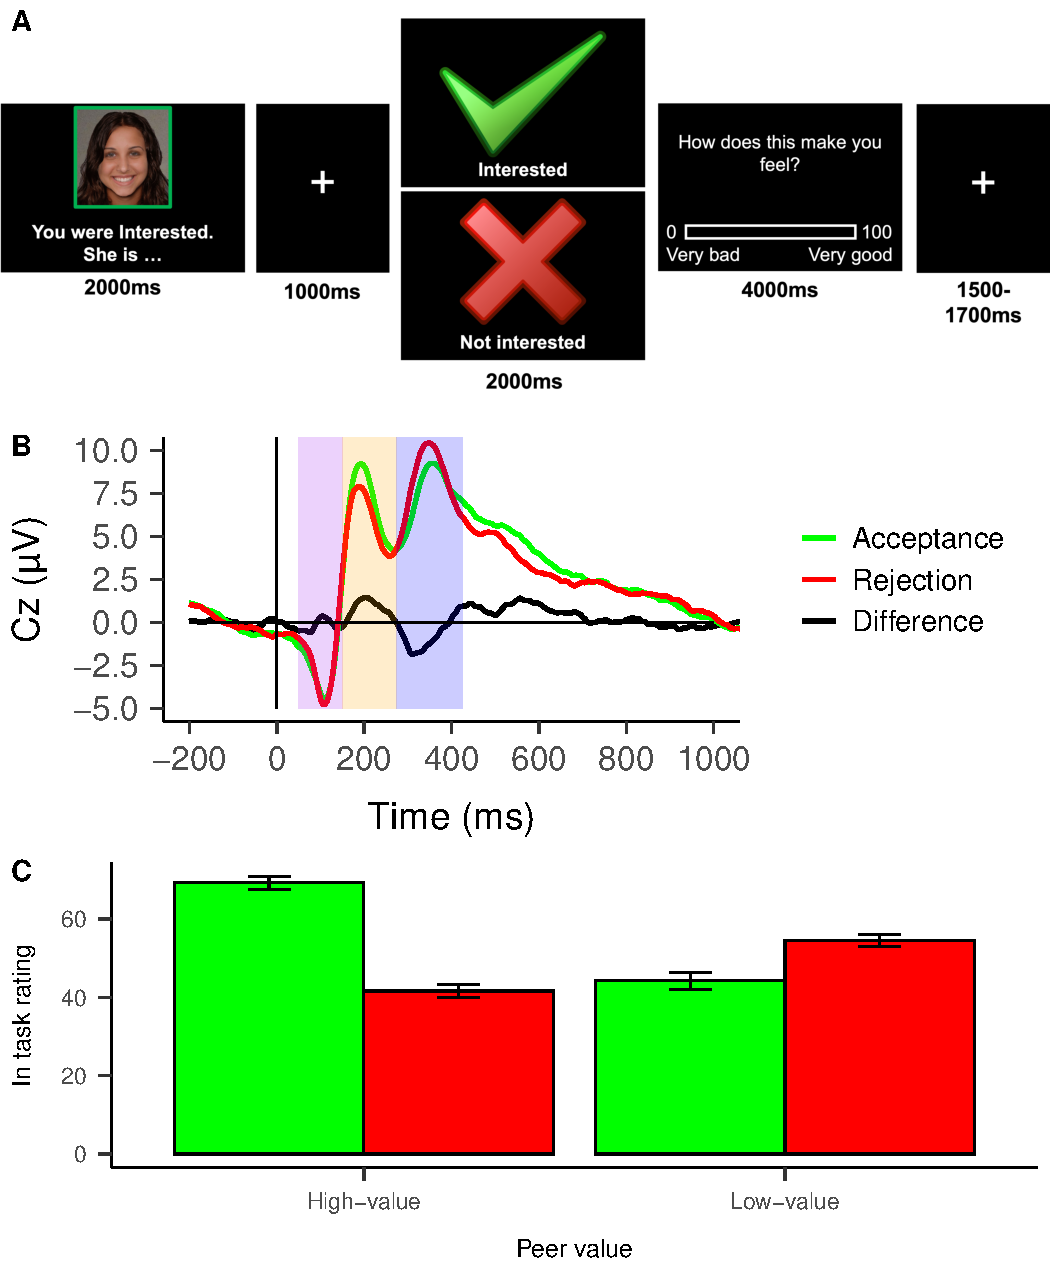
\includegraphics{BUDS_tables_and_figures_working_files/figure-latex/unnamed-chunk-6-1.pdf}
\caption{\label{fig:unnamed-chunk-6}A) Example of trial from chatroom task. B) Grand average ERP for acceptance and rejection feedback from high-value peers. Colored sections of the graph represent time windows where ERP components were extracted at Cz electrode: N1 = purple, RewP = orange, P300 = blue. C) Mean in-task, post-feedback ratings across all participants by Feedback (acceptance, rejection) and Value (high, low).}
\end{figure}

\begin{figure}
\centering
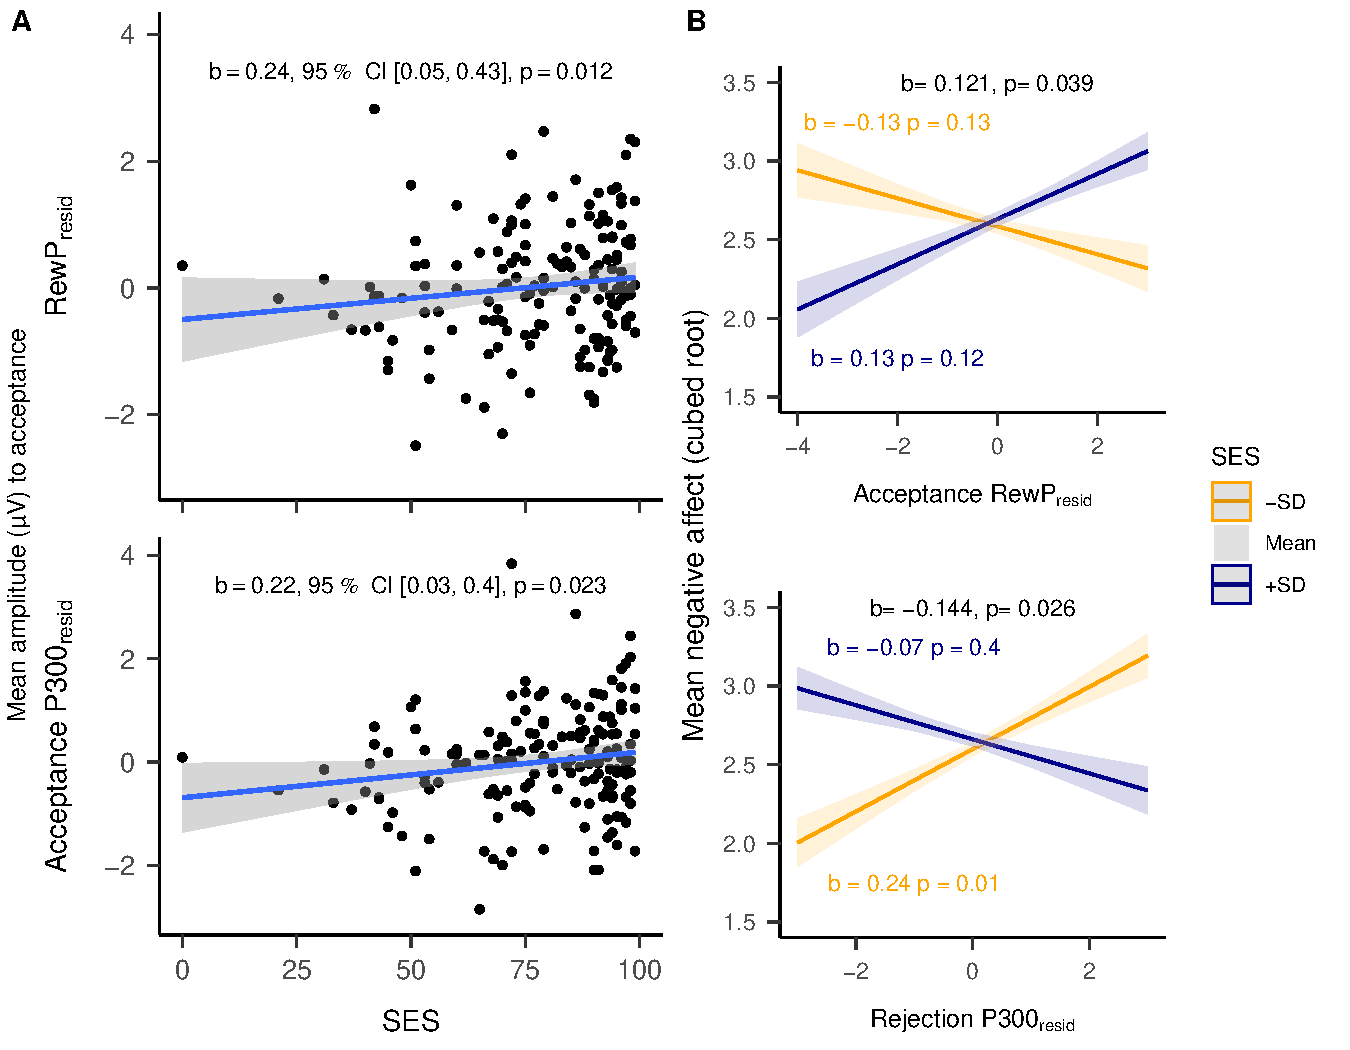
\includegraphics{BUDS_tables_and_figures_working_files/figure-latex/unnamed-chunk-14-1.pdf}
\caption{\label{fig:unnamed-chunk-14}A) Relationship between SES and brain responses to acceptance (relative to rejection) for both the RewP and P300 ERP components. B) Interactions for which SES significantly moderated associated between brain responses to acceptance or rejection and negative affect. RewP: no simple slopes significant. P300: simple slope significant for SES -1 standard deviation below the mean. Note: All plots use residualized scores, such that responses ``Acceptance RewP'' indicates responses to acceptance residualized for rejection, and vice versa.}
\end{figure}

\begin{figure}
\centering
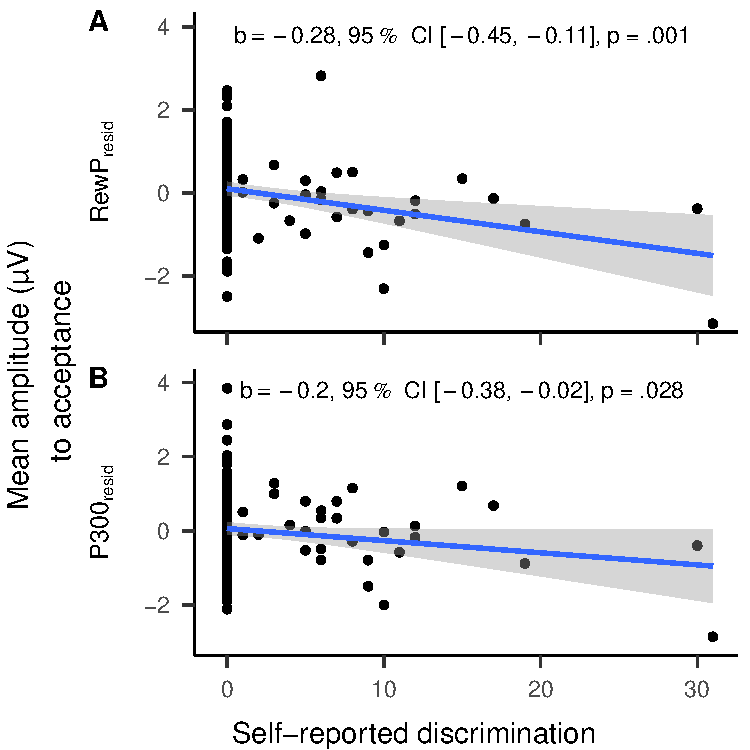
\includegraphics{BUDS_tables_and_figures_working_files/figure-latex/unnamed-chunk-18-1.pdf}
\caption{\label{fig:unnamed-chunk-18}Relationship between SES and brain responses to acceptance (relative to rejection) for both the RewP and P300 ERP components.}
\end{figure}


\end{document}
